\documentclass[conference]{IEEEtran}
\usepackage{cite}
\usepackage{enumitem}
\usepackage{graphicx}
\usepackage{subcaption}
\usepackage{listings}
\usepackage[hyphens]{url}
\usepackage[hidelinks,pdfusetitle]{hyperref}
\usepackage{xcolor}
\usepackage{siunitx}

\hypersetup{
    breaklinks=true,
    pdfauthor={Diogo Medeiros}
}
\urlstyle{same}

\def\BibTeX{{\rm B\kern-.05em{\sc i\kern-.025em b}\kern-.08em
    T\kern-.1667em\lower.7ex\hbox{E}\kern-.125emX}}
    
\lstdefinestyle{mystyle}{
    breakatwhitespace=false,
    breaklines=true,
    captionpos=b,
    keepspaces=true,
    showspaces=false,
    showstringspaces=false,
    showtabs=false,
    tabsize=2
}
\lstset{style=mystyle}

\begin{document}

\title{Icon Generation with Conditional Generative Adversarial Networks}

\author{\IEEEauthorblockN{Diogo Medeiros}
\IEEEauthorblockA{\textit{School of Science and Technology} \\
\textit{University of Trás-os-Montes and Alto Douro}\\
Vila Real, Portugal \\
al70633@alunos.utad.pt}
}
\maketitle

\begin{abstract}
Conditional Generative Adversarial Networks (cGANs) were used to generate icons with specific characteristics or properties given the Icons-50 dataset. The performance of the cGANs was impacted by the imbalanced nature of the original dataset. Filtering the original dataset to include only the 10 most frequent classes (the Icons-10 dataset) improved the performance of the cGANs, allowing them to generate more detailed and striking icons. This paper demonstrates the potential of cGANs for use in applications where a large number of icons with specific characteristics are needed.
\end{abstract}

\begin{IEEEkeywords}
GAN, cGAN, Icons-50, icons, style, applications
\end{IEEEkeywords}

\section{Introduction}
\subsection{Background}
Conditional Generative Adversarial Networks (cGANs) \cite{Mirza2014} are a variant of Generative Adversarial Networks (GANs) that allow the generation of new data samples with specific properties or characteristics. They consist of two neural networks: a generator and a discriminator. The generator is trained to generate new data samples that are similar to a training set, while the discriminator is trained to distinguish between real and fake data samples.

cGANs introduce an additional input to the generator and discriminator networks, known as the conditioning variable, which allows the model to generate data with specific characteristics or properties. This can be useful in a variety of applications, such as image generation, text generation, and speech generation, where the output data needs to have specific attributes or features \cite{Mirza2014}.

For example, in image generation, the conditioning variable may be a label indicating the class of the image to be generated (e.g., a specific type of animal or object), or it may be an attribute of the image (e.g., the presence or absence of a certain color).

\subsection{Problem}
Given a public dataset, Icons-50 \cite{Icons50, Hendrycks2018}, comprised of icons and their respective labels, I want to be able to generate a new set of sample icons corresponding to a specific label, such as ``clock" or ``airplane".

This could be useful in applications where a large number of icons with specific characteristics are needed, such as in user interface design or graphics design.

\subsection{Objective}
Using cGANs, it is possible to generate icons with specific characteristics or properties, given a public dataset such as Icons-50. To do this, the cGAN would be trained on said dataset, with the conditioning variable being the desired label of the generated icons, in this case represented by an integer value corresponding to a class of icons, such ``cat" or ``bird".

\subsection{Related Work}
In Mirza and Osindero \cite{Mirza2014}, the authors introduce the concept of conditional generative adversarial networks (cGANs), which are a variant of generative adversarial networks (GANs) that allow the generation of new data samples with specific properties or characteristics. The cGANs are constructed by feeding the data and the desired characteristics or properties to both the generator and discriminator networks. The authors demonstrate the use of cGANs for generating MNIST digits conditioned on class labels and for learning a multi-modal model. They also provide examples of using cGANs for image tagging, where the model is able to generate descriptive tags that are not part of the training labels.

In Liu et al. \cite{Liu2021SCCGAN:CGAN}, the authors propose a cGAN-based method for repairing damaged fonts based on style. They use the content accuracy and style similarity of the repaired font as evaluation indices to assess the accuracy of the restored style. The results show that the cGAN-based method is able to repair damaged fonts in a way that is similar to the correct content.

In Loey et al. \cite{Loey2020AImages}, the authors propose the use of classical data augmentation techniques along with a cGAN based on a deep transfer learning model for COVID-19 detection in chest CT scan images. The motivation for this research was the limited availability of benchmark datasets for COVID-19, particularly in chest CT images. To address this, the authors collected all available images for COVID-19 and used classical data augmentation techniques along with a cGAN to generate additional images to help in the detection of the virus. The results showed that the classical data augmentation techniques along with the cGAN improved the performance of classification in all selected models.

In Ma et al. \cite{Ma2018SpeckleCGAN}, the authors propose an end-to-end framework based on a cGAN for simultaneously reducing speckle noise and enhancing contrast in retinal OCT images. The cGAN is trained using a novel method for obtaining clean images from outputs of commercial OCT scanners, and an edge loss function is added to the final objective to ensure that the model is sensitive to edge-related details. The results show that the proposed method outperforms traditional and other deep learning methods in terms of denoising performance, and has good generalization ability for different types of retinal OCT images.

\section{Materials and Methods}

\subsection{Data}
To achieve my goal, I opted for the public dataset ``Icons-50" \cite{Icons50}, first introduced in \cite{Hendrycks2018}. According to the authors, this dataset was initially designed to test the robustness of classifiers to surface variations in objects. The dataset includes both new styles of known objects and unexpected instances of known classes, and the authors propose two methods to improve the surface variation robustness of classifiers.

The Icons-50 dataset consists of 10,000 images belonging to 50 classes of icons (e.g., people, food, activities, places, objects, symbols, etc.) collected from different technology companies and platforms (e.g., Apple, Samsung, Google, Facebook, etc.). 

Each class has icons with different styles (e.g., Microsoft's flat vector graphics icon style) and different class sub-types (e.g., 'duck' or 'eagle' sub-types in the 'birds' class) \cite{Icons50}.

To summarize, each entry in the dataset is comprised of the following parameters:
\begin{itemize}
    \item image - a 3x32x32 NumPy array corresponding to the RGB icon
    \item class - an integer between 0 and 49 representing the icon's class
    \item sub-type - a string corresponding to the class sub-type, e.g., ``broken\_heart" for the class ``heart" (label 26)
    \item style - a string corresponding to the icon's source, such as Microsoft or Apple
    \item rendition - an integer between 0 and 9 representing the icon's version
\end{itemize}

When analyzing the class distribution, I came to the conclusion that the Icons-50 dataset was considerably unbalanced, as seen in Fig.~\ref{fig:Icons50ClassDist}.

\begin{figure}[htbp]
    \centering
    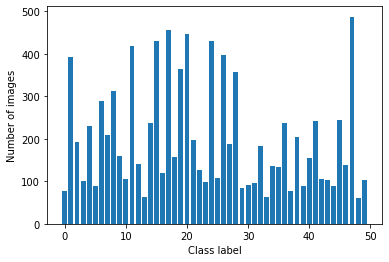
\includegraphics[width=0.48\textwidth]{paper/images/icons50/class_dist.png}
    \caption{Class distribution of the Icons-50 dataset}
    \label{fig:Icons50ClassDist}
\end{figure}

This led to the creation of Icons-10, a subset of Icons-50 containing the top 10 most frequent classes in the dataset, with the old labels mapped to new values between 0 and 9. The Icons-10 dataset comprises 4170 images and has a fairly balanced class distribution, seen both in Fig.~\ref{fig:Icons10ClassDist} and in Table~\ref{tab:Icons10Desc}.

\begin{figure}[htbp]
    \centering
    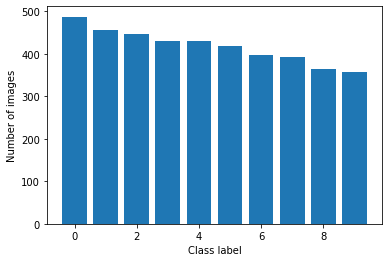
\includegraphics[width=0.48\textwidth]{paper/images/icons10/class_dist.png}
    \caption{Class distribution of the Icons-10 dataset}
    \label{fig:Icons10ClassDist}
\end{figure}

\begin{table}[htbp]
    \centering
    \caption{Icons-10 Dataset}
    \begin{tabular}{cccc}
    \hline
    \textbf{Class} & \textbf{Old label} & \textbf{New label} & \textbf{No. samples} \\ \hline
    worker & 47 & 0 & 487  \\ 
    family & 17 & 1 & 455  \\
    flag & 20 & 2 & 446  \\
    face & 15 & 3 & 429  \\
    hands & 24 & 4 & 429  \\
    clock & 11 & 5 & 417  \\
    heart & 26 & 6 & 396  \\
    arrow & 1 & 7 & 392  \\
    cat & 19 & 8 & 363  \\
    ideograph & 28 & 9 & 356 \\ \hline
    \end{tabular}
    \label{tab:Icons10Desc}
\end{table}

\subsection{Methods}
I opted to adapt an already existing implementation of a cGAN model using the \texttt{keras} library, with the original source code available in \cite{BrownleeCGAN, BrownleeGAN}. In the original post, the author chooses to train the model with the MNIST Fashion dataset, which is comprised of gray-level images with 28x28 pixels, far different from the Icons-50 dataset specifications.

In the case of a regular GAN, in Fig.~\ref{fig:GANArch}, the generator takes in the input vector randomly drawn from the latent space and outputs the generated image, which is fed to the discriminator, along side real examples from the dataset, and outputs a classification: whether or not it is real.

\begin{figure}[htbp]
    \centering
    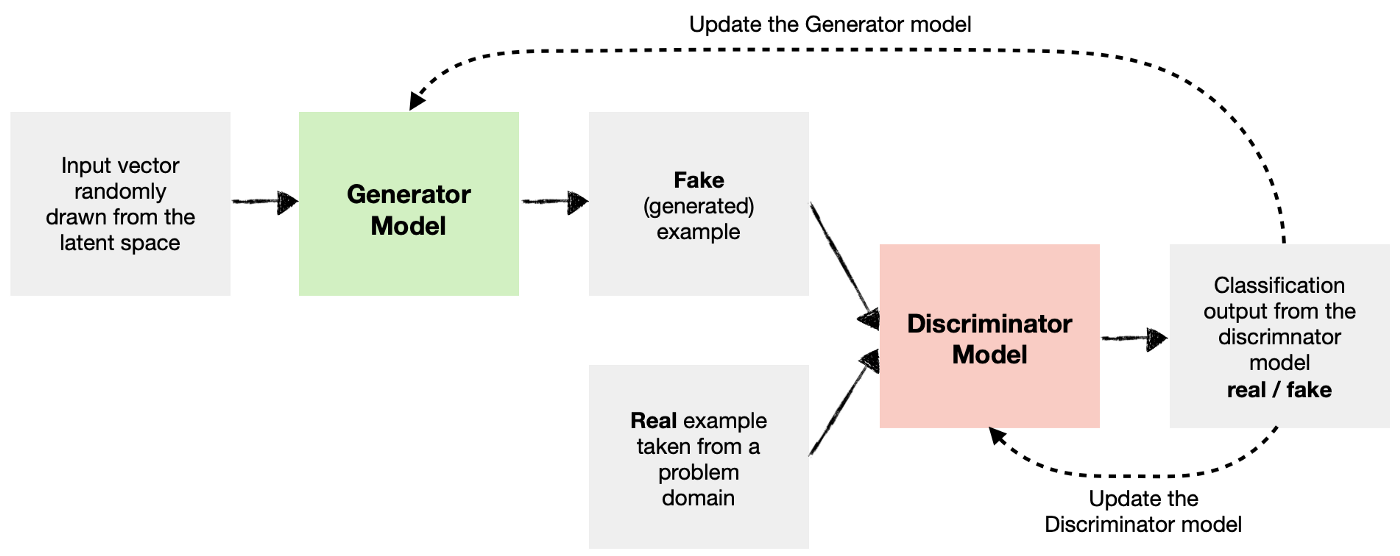
\includegraphics[width=0.48\textwidth]{paper/images/architecture/gan_arch.png}
    \caption{Architecture of traditional Generative Adversarial Networks (GANs)}
    \label{fig:GANArch}
\end{figure}

The main difference between the regular GAN and the cGAN models can be seen in Fig.~\ref{fig:cGANArch}. The conditioning variable, in this case, is the icon's class label, which is fed both to the generator when generating a new fake icon, and to the discriminator in order to learn whether or not it belongs to the specific class.

\begin{figure}[htbp]
    \centering
    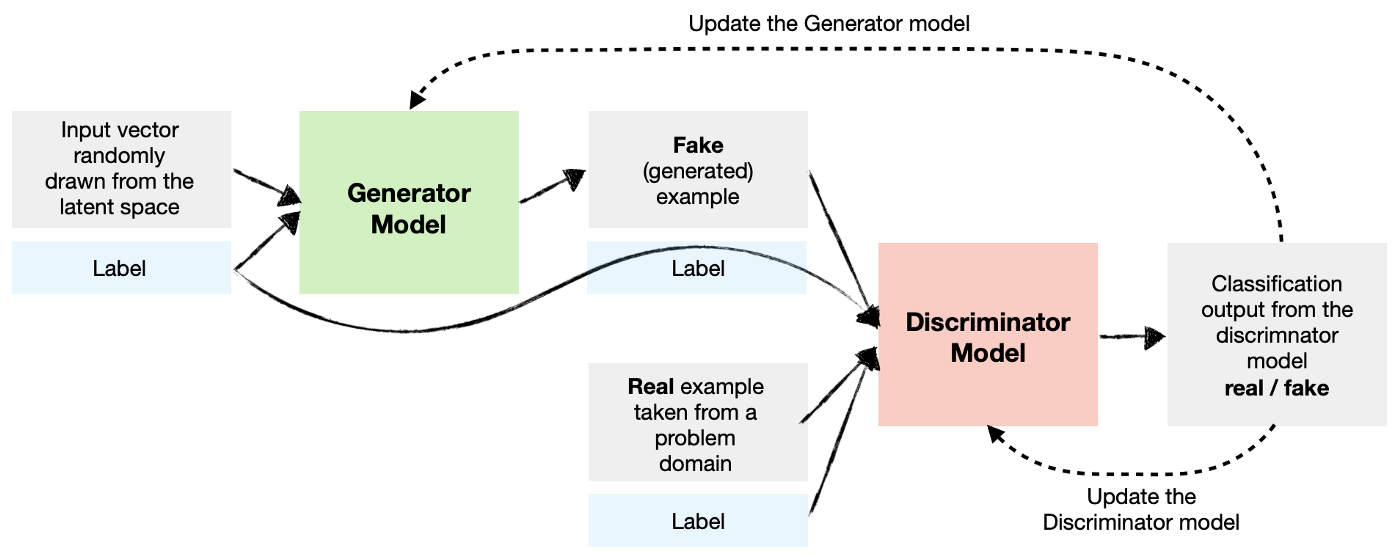
\includegraphics[width=0.48\textwidth]{paper/images/architecture/cgan_arch.png}
    \caption{Architecture of Conditional Generative Adversarial Networks (cGANs)}
    \label{fig:cGANArch}
\end{figure}

With all this in mind, I built the model, starting with the generator. 

As it is clear from Fig.~\ref{fig:GenStruct}, the generator takes in the class label of the icon I want to generate and an input vector drawn randomly from the latent space, with a dimension set at 100. It has a total of 1.38M parameters.

In terms of the activation layers, I opted for the leaky ReLU with an alpha of 0.2, apart from the output layer with a \textit{tanh} activation.

\begin{figure}[htbp]
    \centering
    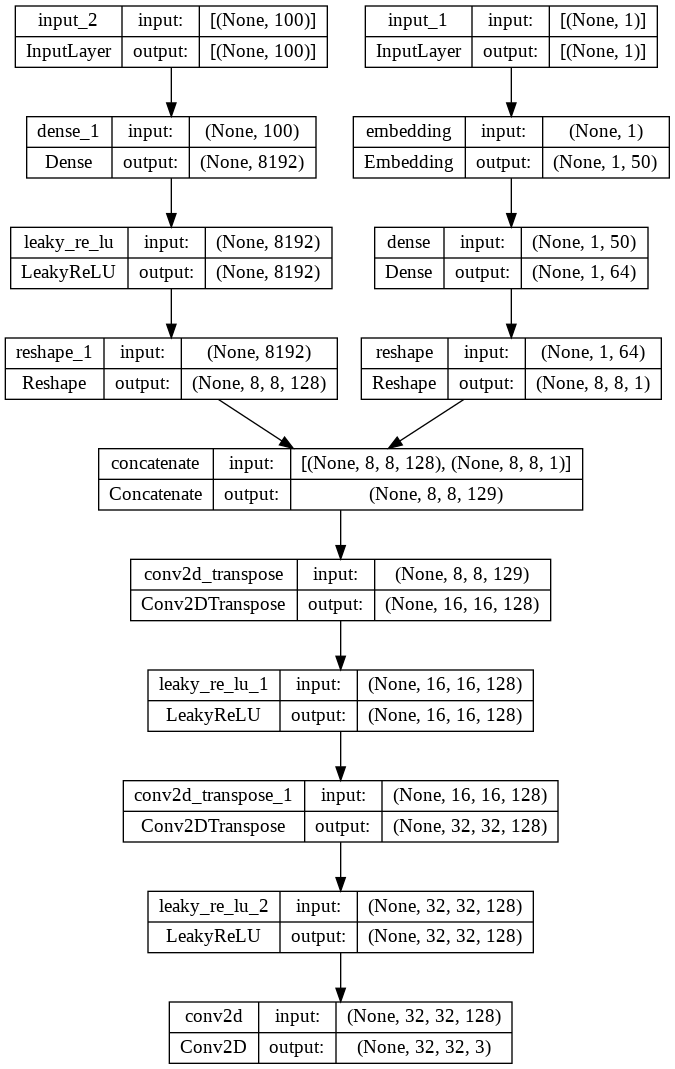
\includegraphics[width=0.4\textwidth]{paper/images/summary/generator.png}
    \caption{Structure of the generator model}
    \label{fig:GenStruct}
\end{figure}

Now for the discriminator, as it is evident from (Fig.~\ref{fig:DiscStruct}), I again chose the leaky ReLU function with an alpha of 0.2 for most model layers, apart from the output, which in this case has a \textit{sigmoid} activation, as I are dealing with a binary classification problem.

Since the discriminator is to be trained individually, it must be compiled with a given optimizer, in this case, the Adam optimizer, with a learning rate $LR=\num{2e-4}$ and a $\beta_1=0.5$. It has a total of 0.22M parameters.

\begin{figure}[htbp]
    \centering
    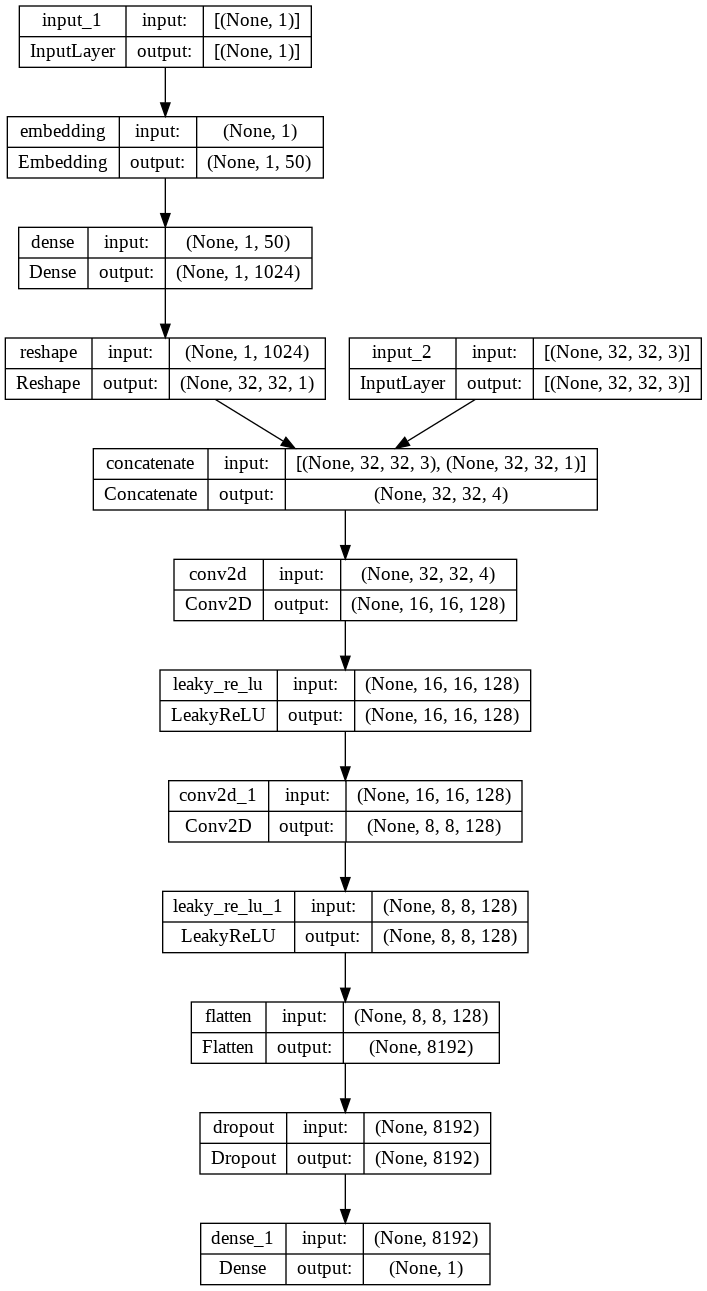
\includegraphics[width=0.4\textwidth]{paper/images/summary/discriminator.png}
    \caption{Structure of the discriminator model}
    \label{fig:DiscStruct}
\end{figure}

Finally, I assemble the cGAN model by taking the generator's output and the input class label and feeding them to the discriminator, as seen in Fig.~\ref{fig:cGANStruct}.

\begin{figure}[htbp]
    \centering
    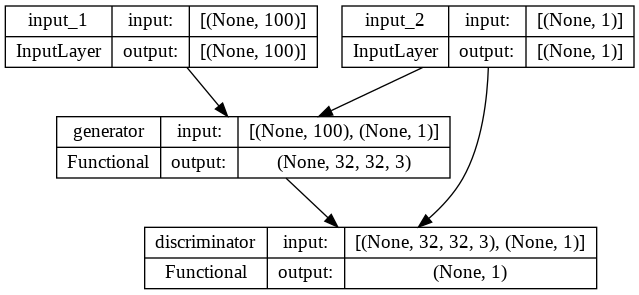
\includegraphics[width=0.48\textwidth]{paper/images/summary/cgan.png}
    \caption{Structure of the cGAN model}
    \label{fig:cGANStruct}
\end{figure}

I chose to train trained two models with identical architectures, first with the original dataset, the Icons-50, and then with the new Icons-10 subset. Given the smaller dataset, I picked an appropriate batch size to match its length, seen in Table~\ref{tab:ModelParams}.

\begin{table}[htbp]
    \centering
    \caption{Model parameters}
    \begin{tabular}{ccccc}
    \hline
    \textbf{Dataset} & \textbf{Parameters} & \textbf{Epochs} & \textbf{Batch Size} & \textbf{Latent Dim} \\ \hline
    Icons-50 & 1.6M & 100 & 50 & 100 \\
    Icons-10 & 1.6M & 100 & 30 & 100 \\ \hline
    \end{tabular}
    \label{tab:ModelParams}
\end{table}

\section{Results}

After training the model with the Icons-50 dataset for 100 epochs, I was able to achieve a remarkable classification accuracy on the discriminator, seen in Fig.~\ref{fig:Icons50Acc}, with a 94\% accuracy for real images and a 98\% accuracy for generated images.

\begin{figure}[htbp]
    \centering
    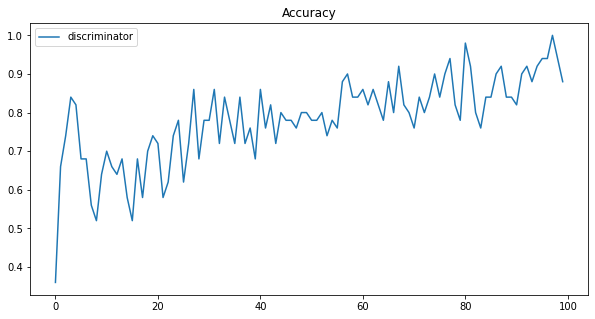
\includegraphics[width=0.48\textwidth]{paper/images/icons50/icons50_acc.png}
    \caption{Discriminator accuracy on the Icons-50 dataset}
    \label{fig:Icons50Acc}
\end{figure}

In terms of loss, while the discriminator finished with a satisfactory minimal loss of 0.329, the same could not be said for the generator, as its loss kept increasing as the training went along, finishing at a value of around 2.532, as can be seen in Fig.~\ref{fig:Icons50Loss}.

\begin{figure}[htbp]
    \centering
    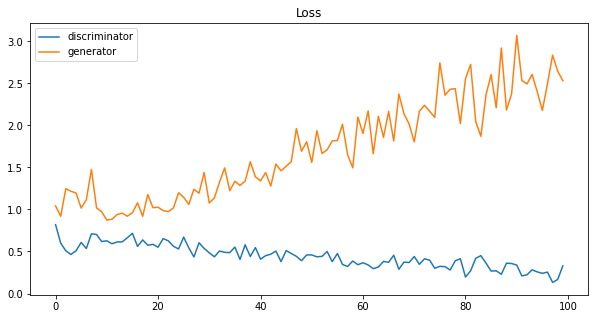
\includegraphics[width=0.48\textwidth]{paper/images/icons50/icons50_loss.png}
    \caption{Model loss on the Icons-50 dataset}
    \label{fig:Icons50Loss}
\end{figure}

Afterwards, I trained a new model, with the same structure, on the Icons-10 subset, again for 100 epochs. When analyzing the discriminator's performance, it seemed that both its loss and accuracy suffered. 

While the loss only increased slightly, to an acceptable value of 0.643, the accuracy while classifying images as real or fake varied quite drastically during training, as can be seen on Fig.~\ref{fig:Icons10Acc}, finishing at, respectively, 83.33\% and 86.67\%.

\begin{figure}[htbp]
    \centering
    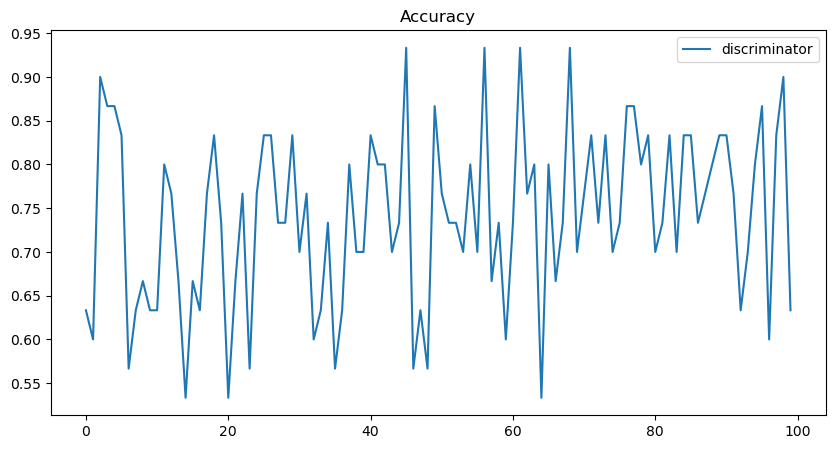
\includegraphics[width=0.48\textwidth]{paper/images/icons10/icons10_acc.png}
    \caption{Discriminator accuracy on the Icons-10 dataset}
    \label{fig:Icons10Acc}
\end{figure}

In terms of the generator's performance, while the loss still varied quite significantly, the the new dataset proved successful, with the model finishing with a much better loss of 1.433, as seen on Fig.~\ref{fig:Icons10Loss}.

\begin{figure}[htbp]
    \centering
    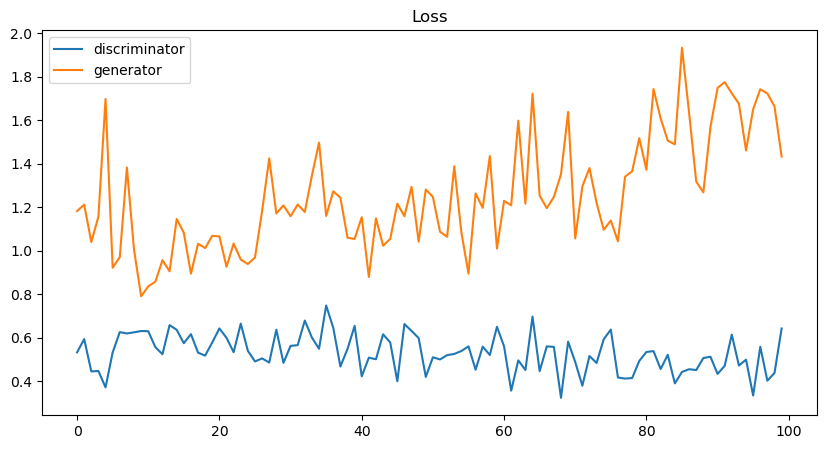
\includegraphics[width=0.48\textwidth]{paper/images/icons10/icons10_loss.png}
    \caption{Model loss on the Icons-10 dataset}
    \label{fig:Icons10Loss}
\end{figure}

To better evaluate the performance of the trained generators, I generated a new set of icons belonging to the classes common to both datasets.

\begin{figure}[htbp]
    \begin{subfigure}[h]{0.4\linewidth}
        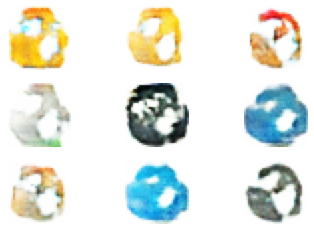
\includegraphics[width=\linewidth]{paper/images/gen_icons/icons50_clock.png}
        \caption{Icons-50 dataset}
        \label{fig:Icons50Clock}
    \end{subfigure}
    \hfill
    \begin{subfigure}[h]{0.4\linewidth}
        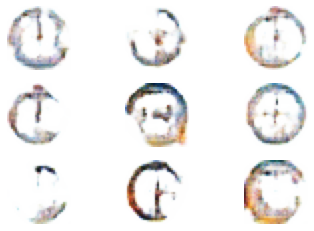
\includegraphics[width=\linewidth]{paper/images/gen_icons/icons10_clock.png}
        \caption{Icons-10 dataset}
        \label{fig:Icons10Clock}
    \end{subfigure}
    \caption{Generated icons belonging to class ``clock"}
    \label{fig:ClockIcons}
\end{figure}

When given a simple task, such as generating a ``clock" icon, the model trained on the Icons-50 dataset only seemed to perceive the shape of the clock, with none of the defining details being present in the generated images, evident from Fig.~\ref{fig:Icons50Clock}.

The second model performed much better on this task, capturing finer details such as the correct color, and the hour and minutes hands, as it is clear from Fig.~\ref{fig:Icons10Clock}.

\begin{figure}[htbp]
    \begin{subfigure}[h]{0.4\linewidth}
        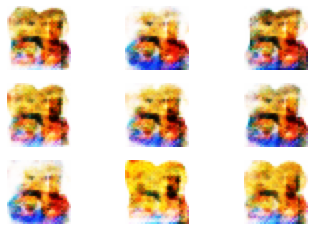
\includegraphics[width=\linewidth]{paper/images/gen_icons/icons50_family.png}
        \caption{Icons-50 dataset}
        \label{fig:Icons50Family}
    \end{subfigure}
    \hfill
    \begin{subfigure}[h]{0.4\linewidth}
        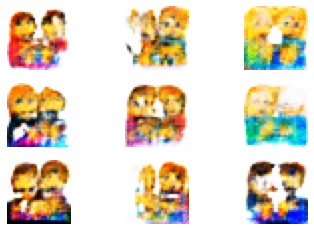
\includegraphics[width=\linewidth]{paper/images/gen_icons/icons10_family.png}
        \caption{Icons-10 dataset}
        \label{fig:Icons10Family}
    \end{subfigure}
    \caption{Generated icons belonging to class ``family"}
    \label{fig:FamilyIcons}
\end{figure}

When dealing with a complex task, such as generating icons for the ``family" class, the original generator was able to create recognizable images, even though they lacked definition and variability, as seen on Fig.~\ref{fig:Icons50Family}. 

When trained on the Icons-10 dataset, the model was able to generate a unique and slightly more detailed set of icons, albeit with variable results, as seen on Fig.~\ref{fig:Icons10Family}.

\section{Discussion}

When dealing with imbalanced data, such as the Icons-50 dataset, it is important to consider how this may impact the training of a machine learning (ML) model, especially when the number of classes is large.

When trained with the original unfiltered data, the discriminator was able to achieve a high accuracy of around 96\% and a small loss of 0.329. While these results would be optimal in their own, when analyzed alongside the generator's performance, the model seemed to overfit the data, possibly due to the large number of classes, finishing off with a disappointing loss of 2.532.

Afterwards, I decided to filter out the dataset by choosing the 10 most frequent classes, in the hope that when training a new model, I would be able to achieve better results when it came to the icon generation. I called this new dataset, fittingly, the Icons-10 dataset.

I then trained a new model with an identical structure to the first one, but now on the filtered data. As to be expected, while the discriminator suffered a slight dip in performance, with an accuracy of 85\% and a loss of 1.433, the generator improved quite significantly, with a lower loss of 1.433.

When analyzing the icons generated by each model, it became apparent that, while the first model was able to learn the overall structure and element composition of the icon, particularly in the case of the ``family" class, the results were lackluster and lacked the proper detail to discern what they represented, without the added context, as seen in Fig.~\ref{fig:Icons50Clock},\ref{fig:Icons50Family}.

This suggests that the generator may not have been deep or large enough to learn the necessary features for generating icons for 50 different classes, while the model trained with the Icons-10 dataset was able to learn and generated detailed and striking images, such as Fig.~\ref{fig:Icons10Clock},\ref{fig:Icons10Family}.

\section{Conclusions}
In this paper, the ability of conditional generative adversarial networks (cGANs) to generate icons with specific characteristics or properties was explored using the Icons-50 dataset. To address the issue of imbalanced data in the original unfiltered dataset, a new dataset was created by filtering the original dataset to include only the 10 most frequent classes (the Icons-10 dataset). 

When comparing the performance of the cGANs trained on these two datasets, it was found that the model trained on the Icons-10 dataset was able to generate more detailed and striking icons compared to the model trained on the unfiltered data. This suggests that the model trained on the Icons-10 dataset was able to learn more effectively and generate more accurate and representative icons for the desired classes.

In conclusion, cGANs can be an effective tool for generating icons with specific characteristics or properties, given a suitable dataset. In this case, filtering the original dataset to include only the most frequent classes improved the performance of the cGANs, demonstrating the importance of considering the impact of imbalanced data on model training. 

Future work could include testing the performance of cGANs with different hyper-parameters or architectures, or using a different dataset with more balanced class distribution. Additionally, exploring the use of cGANs for generating icons with other specific characteristics or properties, such as color or shape, could be a valuable direction for future research

\bibliographystyle{IEEEtran}
\bibliography{paper/references}

\end{document}
